\documentclass{elsart}

\usepackage{graphicx}

\usepackage{amssymb}

\begin{document}

\section{Plotting all figures for Scenario1PullFromEntity}
\subsection{CPU Load}

\begin{figure}[ht]
\centering
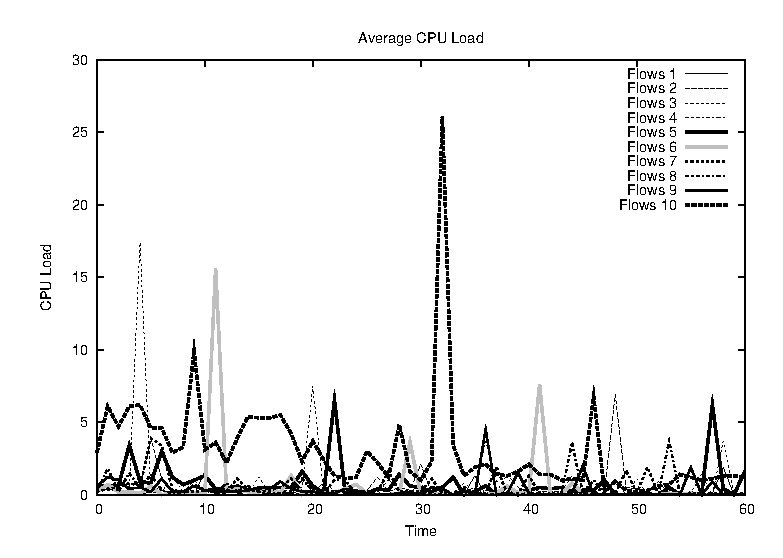
\includegraphics{Scenario1PullFromEntity/cpuload.eps}
\caption{cpuload.eps}\label{fig:cpuload}
\end{figure}

\clearpage
\subsection{Memory State}

\begin{figure}[ht]
\centering
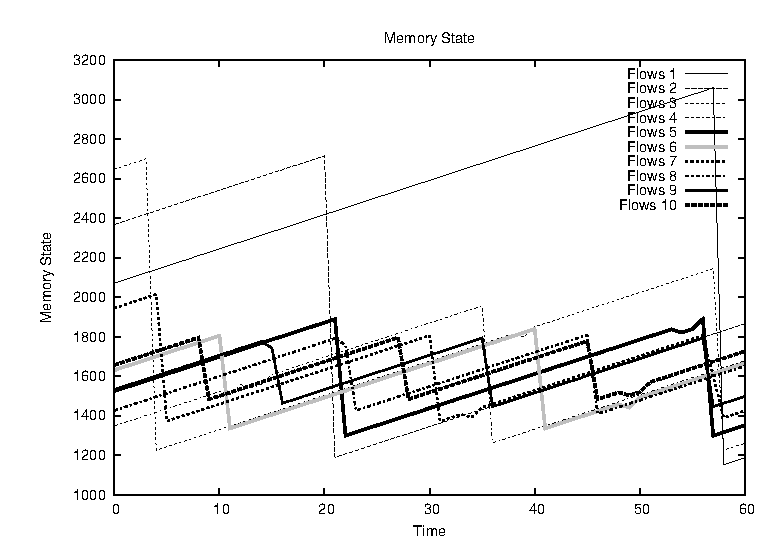
\includegraphics{Scenario1PullFromEntity/memorystorage.eps}
\caption{memorystorage.eps}\label{fig:memorystorage}
\end{figure}

\clearpage
\subsection{Response Time}

\begin{figure}[ht]
\centering
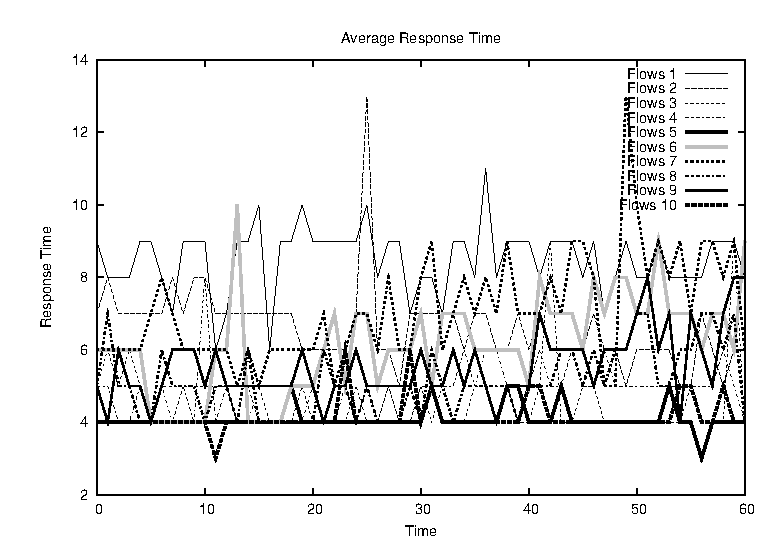
\includegraphics{Scenario1PullFromEntity/responsetime.eps}
\caption{responsetime.eps}\label{fig:responsetime}
\end{figure}

\clearpage
\subsection{Information Freshness}

\begin{figure}[ht]
\centering
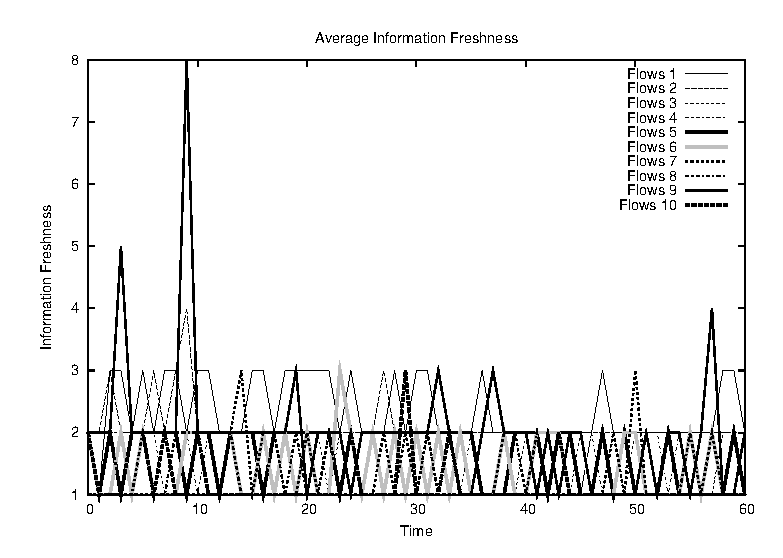
\includegraphics{Scenario1PullFromEntity/freshness.eps}
\caption{freshness.eps}\label{fig:freshness}
\end{figure}

\clearpage
\subsection{Response Time of Selected Flows}

\begin{figure}[ht]
\centering
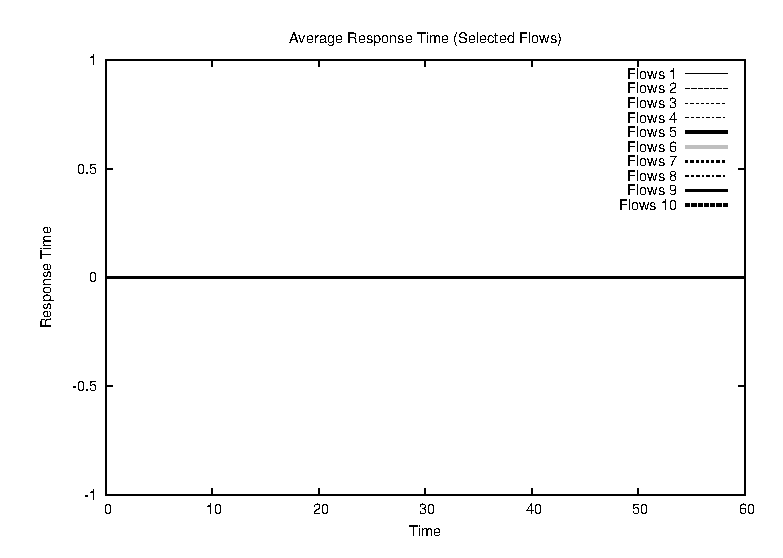
\includegraphics{Scenario1PullFromEntity/responsetimemonitoredflows.eps}
\caption{responsetimemonitoredflows.eps}\label{fig:responsetimemonitoredflows}
\end{figure}

\clearpage
\subsection{Information Freshness of Selected Flows}

\begin{figure}[ht]
\centering
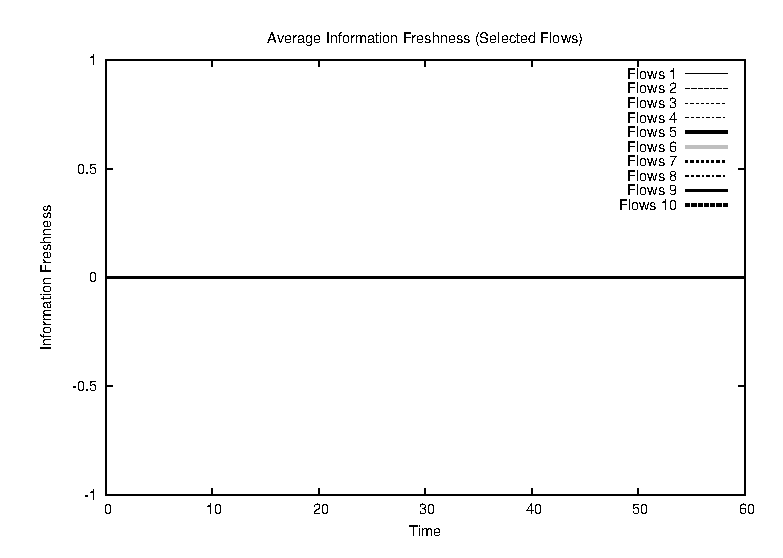
\includegraphics{Scenario1PullFromEntity/freshnessmonitoredflows.eps}
\caption{freshnessmonitoredflows.eps}\label{fig:freshnessmonitoredflows}
\end{figure}

\clearpage

\end{document}
